\documentclass[man,12pt,floatsintext, a4paper, draftfirst]{apa6}\usepackage[]{graphicx}\usepackage[]{color}
%% maxwidth is the original width if it is less than linewidth
%% otherwise use linewidth (to make sure the graphics do not exceed the margin)
\makeatletter
\def\maxwidth{ %
  \ifdim\Gin@nat@width>\linewidth
    \linewidth
  \else
    \Gin@nat@width
  \fi
}
\makeatother

\definecolor{fgcolor}{rgb}{0.345, 0.345, 0.345}
\newcommand{\hlnum}[1]{\textcolor[rgb]{0.686,0.059,0.569}{#1}}%
\newcommand{\hlstr}[1]{\textcolor[rgb]{0.192,0.494,0.8}{#1}}%
\newcommand{\hlcom}[1]{\textcolor[rgb]{0.678,0.584,0.686}{\textit{#1}}}%
\newcommand{\hlopt}[1]{\textcolor[rgb]{0,0,0}{#1}}%
\newcommand{\hlstd}[1]{\textcolor[rgb]{0.345,0.345,0.345}{#1}}%
\newcommand{\hlkwa}[1]{\textcolor[rgb]{0.161,0.373,0.58}{\textbf{#1}}}%
\newcommand{\hlkwb}[1]{\textcolor[rgb]{0.69,0.353,0.396}{#1}}%
\newcommand{\hlkwc}[1]{\textcolor[rgb]{0.333,0.667,0.333}{#1}}%
\newcommand{\hlkwd}[1]{\textcolor[rgb]{0.737,0.353,0.396}{\textbf{#1}}}%
\let\hlipl\hlkwb

\usepackage{framed}
\makeatletter
\newenvironment{kframe}{%
 \def\at@end@of@kframe{}%
 \ifinner\ifhmode%
  \def\at@end@of@kframe{\end{minipage}}%
  \begin{minipage}{\columnwidth}%
 \fi\fi%
 \def\FrameCommand##1{\hskip\@totalleftmargin \hskip-\fboxsep
 \colorbox{shadecolor}{##1}\hskip-\fboxsep
     % There is no \\@totalrightmargin, so:
     \hskip-\linewidth \hskip-\@totalleftmargin \hskip\columnwidth}%
 \MakeFramed {\advance\hsize-\width
   \@totalleftmargin\z@ \linewidth\hsize
   \@setminipage}}%
 {\par\unskip\endMakeFramed%
 \at@end@of@kframe}
\makeatother

\definecolor{shadecolor}{rgb}{.97, .97, .97}
\definecolor{messagecolor}{rgb}{0, 0, 0}
\definecolor{warningcolor}{rgb}{1, 0, 1}
\definecolor{errorcolor}{rgb}{1, 0, 0}
\newenvironment{knitrout}{}{} % an empty environment to be redefined in TeX

\usepackage{alltt}
\usepackage[latin1]{inputenc}
\usepackage{amsmath}
\usepackage{amsfonts}
\usepackage{amssymb}
\usepackage[american]{babel}
\usepackage{csquotes}
\usepackage[style=apa, sortcites=true,url=false, firstinits=true,doi=false,sorting=nyt, backend=biber]{biblatex}
\DeclareLanguageMapping{american}{american-apa}
\usepackage{geometry}
\usepackage{rotating}
\usepackage{graphicx}
\usepackage{units}
\usepackage{multicol}
\usepackage{multirow}
\usepackage{pdflscape}
\usepackage{subcaption}
\usepackage{xfrac}
\usepackage{color}
\usepackage{tikz}
\usepackage{xspace}
\usepackage[textfont=normalfont]{caption}
\usetikzlibrary{arrows,decorations.markings} 
\usetikzlibrary{arrows.meta}
\definecolor{lavendermagenta}{rgb}{0.93, 0.51, 0.93}

%see files osPages.pdf, experiments.pdf, osid.r (constructed from E168/E168a.r, E168/explore.r, E175/e175.r) run vim from rwork vim -S osid.vim
%final osidbf.r/vim
%files for export
%osid/ 		osid#2.Rnw
%			osidbf.Rdata
%			osidBFExport.r
%e168/		osid2Export.r
%			allData168a.Rdata		
%			allData168b.Rdata
%e175/		part1.Rdata
%			part2.Rdata
%functions/ generic.r

\def\pc{/admin/}
%set to spg or admin
\newif\ifsurface
\surfacefalse
%\surfacetrue
%the root r-directory, where common directories and files stored e.g. rwork/functions, rwork/classes
%the data and r-code for the current document will be stored in e.g. rwork/current so functions could be accessed ../functions
\def\rroot{c:/users\pc documents/rwork/}
%define the latex root directory where bibliography stored and where latex /work directory exists
\def\lroot{c:/users\pc documents/latex/}
%pegs stuff needed in some documents
\ifsurface
 \def\proot{D:/Google Drive/PEGS/document/}
 \def\groot{d:/google drive/}
\else
 \def\proot{C:/Users\pc Google Drive/PEGS/document/}
 \def\groot{c:/users\pc google drive/}
\fi

%bibliography
\def\bd{c:/users\pc documents/latex/allbib.bib}
\addbibresource{\bd}

\AtEveryBibitem{% Clean up the bibtex rather than editing it see http://codydunne.blogspot.co.uk/2012/01/suppressing-bibtex-fields-for-specific.html
 \clearfield{note}
 \clearfield{number}
 \clearfield{month}
} 

\newcommand{\trw}{the Rescorla-Wagner model\xspace}
\newcommand{\Trw}{The Rescorla-Wagner model\xspace}
\newcommand{\trrw}{the reduced Rescorla-Wagner model\xspace}
\newcommand{\Trrw}{The reduced Rescorla-Wagner model\xspace}
\newcommand{\tpcm}{the Pearce configural model\xspace}
\newcommand{\Tpcm}{The Pearce configural model\xspace}
\newcommand{\rw}{Rescorla-Wagner\xspace}
\newcommand{\rwm}{Rescorla-Wagner model\xspace}
\newcommand{\cm}{configural model\xspace}
\newcommand{\tcm}{the configural model\xspace}
\newcommand{\Tcm}{The configural model\xspace}
\newcommand{\trhs}{the right-hand side\xspace}
\newcommand{\tlhs}{the left-hand side\xspace}
\newcommand{\rhs}{right-hand side\xspace}
\newcommand{\lhs}{left-hand side\xspace}
\newcommand{\ssr}{smaller-sooner reward\xspace}
\newcommand{\llr}{larger-later reward\xspace}
\newcommand{\dd}{delay-discounting\xspace}
\newcommand{\prz}{preference-reversal-zone\xspace}
\newcommand{\me}{MECA\xspace}
\newcommand{\mem}{MECA model\xspace}
\newcommand{\tme}{the MECA model\xspace}
\newcommand{\Tme}{The MECA model\xspace}
\newcommand{\trme}{the reduced MECA model\xspace}
\newcommand{\Trme}{The reduced MECA model\xspace}
\newcommand{\lli}{log-likelihood\xspace} %suffix i to disambiguate
\newcommand{\llis}{log-likelihoods\xspace}
\newcommand{\ml}{maximum likelihood\xspace}
\newcommand{\Ml}{Maximum likelihood\xspace}
\newcommand{\Cc}{Classical conditioning\xspace}
\newcommand{\cc}{classical conditioning\xspace}
\newcommand{\Pc}{Pavlovian conditioning\xspace}
\newcommand{\cs}{conditioned stimulus\xspace}
\newcommand{\css}{conditioned stimuli\xspace}
\newcommand{\Css}{Conditioned stimuli\xspace}
\newcommand{\us}{unconditioned stimulus\xspace}
\newcommand{\uss}{unconditioned stimuli\xspace}
\newcommand{\Uss}{Unconditioned stimuli\xspace}
\newcommand{\ur}{unconditioned response\xspace}
\newcommand{\urs}{unconditioned responses\xspace}
\newcommand{\Urs}{Unconditioned responses\xspace}
\newcommand{\cri}{conditioned response\xspace} %suffix i to disambiguate
\newcommand{\cris}{conditioned responses\xspace} 
\newcommand{\Cris}{Conditioned responses\xspace}
\newcommand{\mcet}{multiple-context cue-exposure therapy\xspace}
\newcommand{\Mcet}{Multiple-context cue-exposure therapy\xspace}
\newcommand{\mcets}{multiple-context cue-exposure therapies\xspace}
\newcommand{\Mcets}{Multiple-context cue-exposure therapies\xspace}
\newcommand{\cet}{cue-exposure therapy\xspace}
\newcommand{\Cet}{Cue-exposure therapy\xspace}
\newcommand{\cets}{cue-exposure therapies\xspace}
\newcommand{\Cets}{Cue-exposure therapies\xspace}
\usepackage{color}
\usepackage{soul}
\newcommand{\hlc}[2][yellow]{ {\sethlcolor{#1} \hl{#2}} }
\definecolor{bkgdcol}{rgb}{0.86,0.86,0.86}
\definecolor{lavendermagenta}{rgb}{0.93, 0.51, 0.93}


\graphicspath{{../../../../workspace/simlib/}}

\author{Steven Glautier and Ovidiu Brudan}

\affiliation{Southampton University}

\title{Stable Individual Differences in Occasion Setting}
\shorttitle{Differences in Occasion Setting}
\note{6438 words 15/01/18}
\authornote{Correspondence should be addressed to Steven Glautier, School of Psychology, University of Southampton, Southampton, SO17 1BJ, United Kingdom. E-mail: spg@soton.ac.uk, Tel: (+44) 023 8059 2589. Acknowledgements to student volunteer research assistant Jessica Richards for Experiment 1 data collection.}

\abstract{In the current investigation we classified participants as inhibitors or non-inhibitors depending on the extent to which they showed conditioned inhibition in a context that had been used for extinction of a conditioned response. This classification enabled us to predict participant responses in a second experiment which used a different design and a different experimental task. Our results were repeated in two replications and supported by Bayesian analyses. In the second experiment a feature-negative discrimination survived reversal training of the feature to a greater extent in the non-inhibitors than in the inhibitors. We propose that the fundamental distinction between inhibitors and non-inhibitors is based on a tendency to utilise first-order (direct associations) or second-order (occasion-setting) strategies when faced with ambiguous information and that this classification is a stable individual differences attribute.}

\keywords{associative learning, inhibition, occasion-setting, response-recovery, feature-negative discrimination, reversal, individual differences}

\leftheader{Glautier, Brudan}
\IfFileExists{upquote.sty}{\usepackage{upquote}}{}
\begin{document}
\maketitle


\setlength{\parindent}{1cm}
\section{Introduction}
Associative learning plays a crucial role in the survival of organisms by facilitating the acquisition of responses to stimuli which signal significant events. However, acquisition is only half of the story. In an ever-changing environment a response that was once appropriate may become redundant or even maladaptive if it continues to occur when the environmental conditions change. For example an animal may learn that a particular location is a good source of food but if it continues returning to that location after the source is exhausted it will waste energy that could be better spent foraging elsewhere. Procedurally, presenting a \cs (CS) alone, without the \us (US) it was previously paired with, is known as extinction. During extinction the \cri (CR) produced by the CS is observed to decline in magnitude and probability until at some point extinction appears to be complete. Superficially extinction resembles unlearning and in one of the most widely cited theoretical models of associative learning, \trw \parencite{RescorlaWagner1972}, extinction is exactly that -- the undoing, without leaving a trace, of a previously learned association.

However, it is well established that extinction cannot be understood as simple unlearning. Spontaneous recovery and renewal are among those phenomena which demonstrate that traces of the original learning survive extinction \parencite[e.g.][]{Bouton1994}. Spontaneous recovery refers to renewed CRs that occur when the CS is presented after a delay following extinction. \citeauthor{Brooks1993} trained rats with a tone CS signalling delivery of food then presented the CS alone during an extinction phase. Responding clearly declined during extinction. Animals were then given test presentations of the CS either five hours or six days after extinction. Animals tested five hours after extinction showed a slight increase in responding to the CS compared to that seen at the end of extinction. In contrast, animals tested six days after extinction showed dramatically increased responding to the CS compared to that seen at the end of extinction. Actually responding in the test was slightly higher than it was before extinction, a clear spontaneous recovery effect showing that extinction did not simply erase what had been learned during acquisition \parencite{Brooks1993}. Renewal refers to renewed CRs consequent to a contextual changes after extinction. \let\old\postnotedelim \renewcommand{\postnotedelim}{ }\citeauthor[][(Experiment 1)]{BoutonKing1983} \renewcommand{\postnotedelim}{\old} trained rats with a tone CS signalling electric shock in one context, context A (A:T+ trials\footnote{The colon indicates that identifier A refers to a contextual cue. In contrast an undecorated identifier (e.g. T) refers to a discrete cue. When an experiment only involves a single US the  `+' sign indicates a trial with the US and a `-' sign indicates a trial without the US.}), and then extinguished the CS in another context, context B (B:T- trials), before testing the CS back in context A. Clear extinction effects were seen but responding returned when the CS was tested in context A. These results were supported by further tests which showed that the renewal effect was not mediated by the excitatory properties of context A \parencite{BoutonKing1983}. Other rat studies, where testing was carried out in a novel context C (an ABC design as opposed to an ABA design), confirmed that renewal effects do not depend on the excitatory properties of the test context \parencite{BoutonBolles1979}.

Results such as these present important problems for learning theories and in what follows we describe two leading explanations for renewal to set the stage for the experiments to be presented below. The central question is, how we can understand the decline in responding that is seen during extinction when there is clear evidence that the original learning remains intact? We argue that two leading explanations for renewal, one based on context inhibition and one based on occasion-setting, are not mutually exclusive \parencite[e.g.][]{BoutonNelson1994}. The experiments reported below show that human participants may be categorised into one of two groups. In one group, inhibitors, renewal seems to be controlled by inhibitory associations involving the experimental context. In another group, non-inhibitors, we argue that renewal is controlled by an occasion-setting mechanism. The classification of participants into these two groups appears to be relatively stable, allowing predictions to be made across different experimental procedures, and indicates some practical implications. We leave consideration of these practical implications for the Discussion to focus here on two theoretical explanations for renewal.

In associative models learning is conceptualised as changes in the strength of associative links between mental representations of CSs and USs. We review here the operation of \trw as a `standard' model of associative learning \parencite{RescorlaWagner1972}. Although \trw was developed as a model of \Pc in animals its principles are sufficiently general to have been successfully imported into new domains. \Trw has been considered a viable candidate model in a variety of human learning tasks including predictive, causal, and Pavlovian learning \parencite[e.g.][]{DickinsonShanksEtAl1984,Lachnit1988,ChapmanRobbins1990}. In \trw, in the case of simple excitatory learning, where a CS is repeatedly paired with a US, the association strength, $V$, increases towards an asymptote and is greater than zero. When $V>0$ presentation of the CS activates the US representation -- informally presentation of the CS leads to an expectation of the US through spreading activation. However, $V$ may also be less than zero, in which case inhibitory, rather than excitatory learning has taken place. When there is an inhibitory CS-US association presentation of the CS effectively suppresses expectation of the US. Inhibitory learning takes place when an expected US fails to occur and is of particular concern in the current analysis because US expectancy is violated when extinction begins. 

\begin{equation} 
\label{eq:rwSimple} \Delta V=\alpha \beta (\lambda-\Sigma V)
\end{equation}

Equation \ref{eq:rwSimple} is the fundamental \rwm learning equation\label{lab:extstr}. In Equation
\ref{eq:rwSimple} $\Delta V$ is the change in the associative strength between the mental
representation of a predictive stimulus (such as a tone CS) and the representation of the outcome
(such as a shock US) that occurs on a single learning trial. $\Delta V$ is a function of two
learning rate parameters, $\alpha$ for the CS and $\beta$ for the US, and the parenthesised error
term. In the error term $\lambda$ is the value of the US on that trial (usually 1 or 0 for the
occurrence and non-occurrence of the US, respectively) and $\Sigma V$ is the summed associative
strength of all the predictors that are present on the trial. To see how inhibitory learning takes
place during extinction consider the associative strength of cue A after an acquisition phase
involving a series of $A\!:\!A+$ trials. Asymptotically $V_{A:}+V_A \rightarrow 1$ and
$\sfrac{V_{A:}}{V_A}=\sfrac{\alpha_{A:}}{\alpha_A}$. Following acquisition there is an extinction
phase involving $\!B:\!A-$ trials. At the start of extinction $V_{B:}=0$ and $\Sigma V=V_{B:}+V_A>0$.
During extinction $\lambda=0$ and since $\alpha>0$ and $\beta>0$ then $\Delta V <0$. Since
$V_{B:}=0$ at the start of extinction $V_{B:}$ becomes negative during extinction and $V_A$
declines. Learning (and responding) during extinction stops when $V_{B:}+V_A=0$ and at this point $B\!:$
is inhibitory ($V_{B:}<0$) while $A$ remains excitatory ($V_A>0$). The presence of inhibitory $B\!:$ is
said to protect $A$ from extinction.

Despite the fact that the presence of an inhibitory CS during extinction can protect a CS from extinction \parencite[e.g.][]{Rescorla2003} there are few experiments which have found evidence for context inhibition developing during extinction, calling into question the proposal that protection from extinction could occur. In the study mentioned above \citeauthor{BoutonKing1983} used a summation test to look for context inhibition \parencite{BoutonKing1983}. A summation test involves presenting an excitatory cue in compound with a putative inhibitor \parencite{Rescorla1969} and in this case \citeauthor{BoutonKing1983} presented an excitatory CS in the extinction context but no inhibition was detected. More recently \textcite{PolackLabordaEtAl2012} reported evidence for extinction contexts becoming inhibitory in a summation test, and also in a retardation test in which learning is acquired more slowly in the presence of the inhibitor than in its absence \parencite{Rescorla1969}. \citeauthor{PolackLabordaEtAl2012} found clearest evidence for context inhibition during extinction when using short inter-trial-intervals and suggest that this variable may explain why there are few reports of context inhibition in the literature. Again using a summation test but this time using human subjects both \textcite{NelsonSanjuanEtAl2011} and \textcite{HavermansKeukerEtAl2005} found reduced conditioned suppression when an excitatory cue was presented in the extinction context indicating that the context was inhibitory. However, these results are ambiguous since \textcite{NelsonSanjuanEtAl2011} demonstrated that conditioned suppression was also reduced when the excitatory cue was presented in an associatively neutral context. Thus, any putative conditioned inhibitory effect of the extinction context added nothing to conditioned suppression produced by a novel cue-context combination. However, \textcite{Glautier2013a} found clear evidence for context inhibition with appropriate controls using a predictive learning task (see Discussion, page \pageref{lab:previousCI}) so it seems as though it may be premature to rule-out a role for protection from extinction in extinction and renewal effects.

Partly as a result of failures to find extinction context inhibition effects alternatives to the protection from extinction explanation for renewal have been developed. Occasion setters are stimuli that can be shown to influence the expression of an association between a CS and a US without themselves being directly associated with the US. Instead they function by controlling an `and-gate' which switches the CS-US association on or off \parencite{Bouton1994,Holland1992,Swartzentruber1995}. The occasion-setting mechanism is illustrated in Figure \ref{fig:extinctionStructures} where it is contrasted with \trw. Figure \ref{fig:extinctionStructures} shows the hypothesised associative structures that are formed after acquisition (left-hand side) and after extinction (right-hand side). $CS_A$ was paired with the US during an acquisition phase to produce an $A\rightarrow US$ association (left) and then, in a new context, context B,  $CS_A$ was extinguished by presentation without the US. According to \trw, as explained above, this produces an inhibitory association between $CS_A$ and context B (bottom right). In contrast, in the occasion-setting model, it is assumed that context B forms an inhibitory link with the $A\rightarrow US$ structure (top-right) so that when context B is present the association is switched off and switched on otherwise. We term direct associations between CSs and the US `first-order' and associations which operate on first-order associations `second-order'. It should be apparent that renewal of responding is predicted for the second-order model, as well as the first-order model, because when $CS_A$ is presented outside of context B the $A\rightarrow US$ association will be active.\label{lab:extstr1}

The current investigation follows-up the work of \textcite{Glautier2013a}. It was based on an analysis of renewal in which it was assumed that the two mechanisms outlined above could operate. During an extinction phase of a renewal experiment we assumed that participants could suppress responding by conditionalising an $A\rightarrow US$ association that had been learned during the acquisition phase on the experimental context or by learning that the context was inhibitory as illustrated in Figure \ref{fig:extinctionStructures}. In \citeauthor{Glautier2013a}, although there was a clear overall context inhibition effect, approximately 50\% of participants showed some responding to a test cue when it was presented in the extinction context. It was hypothesised that extinction in participants who failed to suppress responding in the extinction context summation test would have had extinction performance controlled by second-order associations. This is because one of the defining features of an occasion-setter is that its occasion-setting function is specific to a particular CS-US relation \parencite[e.g.][]{Holland1989,Holland1992}. Thus, if $B\!:$ has occasion set the $CS_A\rightarrow US$ relation then it should not affect another CS-US relation (e.g. $CS_B\rightarrow US$). In contrast, conditioned inhibition shows no such specificity since it operates on the US representation. Thus, if $B\!:$ has become inhibitory it should suppress responding to any excitatory cue it is compounded with. 

Of course a classification of participants based on a single test has little value unless there is some independent predictive value of that classification. Therefore each of the identically designed experiments reported on below had two parts. Part 1 was a renewal experiment, based closely on \textcite{Glautier2013a}, which provided an inhibition score for each participant. On the basis of these scores participants were classified as inhibitors or non-inhibitors.
In Part 2 participants underwent feature negative training\label{lab:extstr1}, followed by reinforcement of the feature, and then a test to see if the feature negative discrimination was disrupted. It was predicted that the discrimination would be maximally disrupted in the inhibitors, i.e. those predisposed to learn first order solutions. This would be consistent with previous reports which have shown that feature negative discriminations in which the feature is trained as an occasion-setter using serial presentation can be maintained after reinforced trials with the feature \parencite[e.g.][]{Holland1984, Rescorla1987, Holland1992}. The rationalisation of this prediction is illustrated in Figure \ref{fig:reversalStructures}\label{lab:reversalStructures}. After training with $A+$ and $AB-$ trials responding could be controlled by first-order associative structures (left-hand side, bottom) or by second-order structures (left-hand side, top). Following reinforcement of feature $B$ the second-order associative structures formed by the non-inhibitors will have an excitatory input to the US representation from $B$ (right-hand side, top). There is also an excitatory input to the US representation from $A$, but this association is gated closed by the presence of $B$. In contrast the inhibitors will have excitatory inputs to the US representation from both $A$ and $B$ (right-hand side, bottom). Consequently we predicted stronger responses in the $AB$ compound test for the inhibitors than for the non-inhibitors. 



\section{Experiment 1}
Participants took part in a two-part computer-based experiment. Both parts involved predictive learning tasks. Participants viewed a series of on-screen trials and they were told that their task was to learn to predict the outcome of each trial on the basis of visual cues presented at the start of each trial. In Part 1 participants learned to predict coloured flashes on the computer screen on the basis of cues provided in the form of visually distinctive objects which `fell' on each trial from the top to the bottom of the computer screen. Towards the end of the trial, which lasted about 5s, the objects passed a `sensor' located in the bottom part of the screen and the coloured flashes, when they occurred, were timed with and said to be triggered by the object passing the sensor. Participants had to press a key to indicate their expectation, with respect to the coloured flashes, on each trial before the objects passed the sensor. There were three options available; key-R to predicted a red flash, key-G to predict a green flash, or no-key to predict no flash. Participants were instructed to make as many correct predictions as possible but minimise incorrect predictions. Full details of the task are given in \textcite{Glautier2013a}. Part 1 contained acquisition, extinction, and response recovery phases. Responses made in a summation test carried out at the end of the extinction phase were used to classify participants as either non-inhibitors or inhibitors.

In Part 2 participants learned to predict payouts for cards dealt in a fictitious casino game on the basis of visually distinctive symbols and colours borne on each card. Each trial consisted of a `hand' containing one or two cards being `dealt' before the participants adjusted an on-screen indicator to judge the likelihood that the hand would be a winning hand. Ratings were made on an 11-point integer scale ([0\ldots10]) labelled `10 Win', `5=Win or Lose', and `0 Lose'. Participants made their judgements in their own time and were asked to make their judgements as accurate as possible, to reflect the true value of the cards in play. There were no actual payments made for the hands dealt in this task. Once the participants had made their rating the hand was `turned' to reveal whether or not it was a winning hand. Full details of the task are given in \textcite[Experiment 1]{Glautier2013a}. Part 2 contained feature negative training, reversal learning for the feature, and the $AB$ compound test in which we examined differences between the participants classified as either non-inhibitors or inhibitors on the basis of their responses in the summation test from Part 1. Inhibitors were defined as those participants who completely suppressed responding to cue G when it was presented in context B after extinction.

\subsection{Method}
Procedures were approved by the University of Southampton Research Governance Office and the School of Psychology's Ethics Committee.

\subsubsection{Participants}
Twenty-eight participants were recruited by word of mouth by student volunteer research assistant JR from a local community in Wiltshire, UK. Their mean age was 21 years (range 16-30) and they included 11 males. They were paid �4 on completion.

\subsubsection{Apparatus}
The experiment was run on a laptop computer with a screen measuring 30.5 cm x 19.2 cm (W x H). The screen was run at 60hz in 32 bit colour mode with pixel resolutions of 1440 x 900. The display was controlled by a computer programs written by the first author in Microsoft C\# language and used Microsoft XNA Game Studio Version 3.1 for rendering of the experimental scenario.

\subsubsection{Design and procedure}
\label{sec:E1DandP}
Table \ref{tab:designP1} shows the design for Part 1. The columns in the table show the trial types that were presented in each stage of the task. Different stages took place in different contexts wherein the screen background changed. Acquisition, extinction, and the response recovery test took place the three different contexts i.e. it was an ABC design. Characters A, B, C, and G indicate the identity of the cue object that was present on each trial. Characters X, Y, and Z indicate the trial outcomes. The screen backgrounds that served the roles of contexts A:, B:, and C: were selected randomly without replacement from four possibilities for each participant. The cue objects serving the roles of A, B, C, and G were selected randomly without replacement from 16 possibilities for each participant. The coloured flashes serving the roles of X and Y were selected randomly without replacement from two possibilities (red and green) for each participant. Outcome Z designates the no-flash outcome. Trial order was randomised within each stage separately for each participant subject to the constraint that there could be no more that four repeats of a trial type in a single back-to-back sequence.

Table \ref{tab:designP2} shows the design for Part 2. The columns in the table show the trial types that were presented in each stage of the task. Stages were not differentiated by context changes. Characters A, B, C, D, and M represent different cards, the plus and minus signs indicate the outcome, win or lose, that occurred for that trial type. The cards serving the cue roles A, B, C, D, and M were chosen at random without replacement from 182 possibilities for each participant. The 182 possibilities were formed by combination of 14 different foreground symbols and 13 different background colours -- each card was marked with a foreground symbol presented on a background colour. When two cards were presented onscreen their right-left location was randomised. Trial order was randomised within each stage separately for each participant subject to the constraint that there could be no more that four repeats of a trial type in a single back-to-back sequence. We were interested primarily in the feature negative training (A+, AB- trials) but because feature negative discriminations can be solved on the basis of cue cardinality (one cue reinforced, two cues non-reinforced) we included a concurrent feature positive discrimination (C-, CD+ trials) to ensure that participants attended to the identity of the cues.

\subsubsection{Analysis}
Data processing in the Results and Data analyses sections presented below were undertaken using R, JAGS, and associated packages \parencite{Plummer2017,RCDT2012}.






    
\subsection{Results}
\subsubsection{Acquistion, extinction, summation test, and recovery} Figure \ref{fig:AtraceE1} shows the proportion of x-responses made in response to cue A during the acquisition, extinction, and response recovery test phases. The proportion of x-responses increased during the acquisition phase, decreased during extinction, and then recovered on the first trial of the recovery test. The proportion of x-responses to cue A was higher on the first trial of the recovery test than it was on the last block of extinction. Figure \ref{fig:GtraceE1} shows the proportion of x-responses made to cue G during the acquisition and summation test phases. Responses increased during the acquisition phase and were reduced during the summation test.

\subsubsection{Feature negative discrimination and feature reversal} Figure \ref{fig:FNE1} shows that the feature negative and the feature positive discriminations were acquired successfully. The outcome was rated more likely on trials with cue A and on trials with the cue compound CD than on trials with the cue compound AB and on trials with cue C. The reversal training discrimination was also acquired successfully; cue B attracted higher outcome ratings than did cue M (Figure \ref{fig:FNRE1}). Of particular interest was survival of the feature negative discrimination following reversal training. The difference in response to cue A and the cue compound AB after reversal training is shown in Figure \ref{fig:FNTE1} where it can be seen that cue B maintained it's capacity to suppress responses to cue A. Responses to cue A were higher on the A+ reminder trials than on the AB- feature negative survival test trials.

\subsubsection{AB compound test}
Figure \ref{fig:INTE1} shows responses to the AB compound after feature reversal as a function of inhibition group. The Inhibition group produced higher ratings for the outcome than the No-Inhibition group. There were 18 participants classified as inhibitors out of 28.

\section{Experiment 2}
Differences from Experiment 1 are noted below.

\subsection{Method}

\subsubsection{Participants}
Fifty-two participants were recruited from the University of Southampton Highfield campus by word of mouth and posted advertisement. Their mean age was 20.6 years (range 18-39) and they included 13 males. Course credit was given for participation.

\subsubsection{Apparatus}
The experiment was run on personal computers with screens measuring 41 cm x 26 cm (W x H). The screens were run at 75hz in 32 bit colour mode with pixel resolutions of 1440 x 900. 

\subsection{Results}

\subsubsection{Acquistion, extinction, summation test, and recovery} Figure \ref{fig:AtraceE2} shows the proportion of x-responses made in response to cue A during the acquisition, extinction, and response recovery test phases. The proportion of x-responses increased during the acquisition phase, decreased during extinction, and then recovered on the first trial of the recovery test. The proportion of x-responses to cue A was higher on the first trial of the recovery test than it was on the last block of extinction. Figure \ref{fig:GtraceE2} shows the proportion of x-responses made to cue G during the acquisition and summation test phases. Responses increased during the acquisition phase and were reduced during the summation test.

\subsubsection{Feature negative discrimination and feature reversal} Figure \ref{fig:FNE2} shows that the feature negative and the feature positive discriminations were acquired successfully. The outcome was rated more likely on trials with cue A and on trials with the cue compound CD than on trials with the cue compound AB and on trials with cue C. The reversal training discrimination was also acquired successfully; cue B attracted higher outcome ratings than did cue M (Figure \ref{fig:FNRE2}). Of particular interest was survival of the feature negative discrimination following reversal training. The difference in response to cue A and the cue compound AB after reversal training is shown in Figure \ref{fig:FNTE2} where it can be seen that cue B maintained it's capacity to suppress responses to cue A. Responses to cue A were higher on the A+ reminder trials than on the AB- feature negative survival test trials.

\subsubsection{AB compound test}
Figure \ref{fig:INTE2} shows responses to the AB compound after feature reversal as a function of inhibition group. The Inhibition group produced higher ratings for the outcome than the No-Inhibition group. There were 31 participants classified as inhibitors out of 52.

\section{Data analyses}
Two main Bayesian analyses were carried out on the critical data from the AB compound test. The analyses were based on examples given in \textcite{Kruschke2015} and \textcite{LeeWagenmakers2014}. Data was combined over both experiments for these analyses. Bayesian analyses were chosen due to their inherent suitability for sequential updating of parameter estimates over repeated runs of an experiment \parencite{Kruschke2013,WagenmakersLodewyckxEtAl2010,Dienes2011} and to obtain full distributional information on the parameters of interest. Under conventional null-hypothesis-testing combining data across experiments requires special techniques to be applied to avoid inflated Type I error rate \parencite{ArmitageBerryEtAl2002} and the order in which the data comes in can influence the result. In contrast Bayesian approaches are explicitly based upon updating of estimates as each new piece of evidence comes in and the order of data arrival does not affect the final conclusions. The R-code, JAGS model specifications, and raw data to check and reproduce the analyses reported below can be found at \url{link to data and analysis}.

\subsection{Analysis 1}
Figure \ref{tab:gm1} shows a graphical representation of the JAGS model that was used for Analysis 1 in which the posterior distributions for the ratings obtained in the AB compound test were estimated for the non-inhibitor and the inhibitor groups. The ratings of the non-inhibitors ($x_i$) were assumed to come from a Gaussian distribution with mean $\mu$ and standard deviation $\sigma$. The ratings of the inhibitors ($y_i$) were assumed to come from a Gaussian distribution with mean $\mu+\delta$ and standard deviation $\sigma$. The prior on $\mu$ was a Gaussian with mean $\mu_x$ equal to the observed mean from the non-inhibitor group and standard deviation $\sigma_\mu = 100\times \sigma_{xy}$ where $\sigma_{xy}$ was the observed standard deviation pooled across both groups. The prior on $\sigma$ was a uniform distribution over the range $[\sigma_{xy} \times \sfrac{1}{100} \ldots \sigma_{xy} \times 100]$. The prior on $\delta$ was a Gaussian with mean equal to zero and standard deviation $\sigma_\delta = 100 \times \sqrt{2} \times \sigma_{xy}$. Using $\sqrt{2}$ is based on the fact that the variance of difference between two normally distributed random variables $x$ and $y$ is $\sigma_x^2 + \sigma_y^2$ \parencite{Weisstein2017}, therefore the standard deviation of the difference between two normally distributed random variables $x$ and $y$, both of which have standard deviation $\sigma_{xy}$, is $\sqrt{2} \times \sigma_{xy}$. Given these priors a JAGS model was run with three chains, each with randomly generated initial values (within constraints), over 50000 iterations discarding the first 5000 `burn-in' samples. The chains were observed to converge and the posterior distributions presented in Figure \ref{fig:posteriors} were constructed by pooling across chains.

The means of the posterior distributions shown in Figure \ref{fig:posteriors} for the non-inhibitor and inhibitor group ratings were 1.08 ($\mu$) and 2.54 ($\mu+\delta$) respectively and the common standard deviation ($\sigma$) estimated for both groups was 2.53. To answer the question of whether or not the ratings differed for the non-inhibitors and inhibitors we can consider the region of practical equivalence (ROPE) around the mean of the posterior for the non-inhibitors and the 95\% credible interval around the mean of the posterior for the inhibitors \parencite{Kruschke2015}. The ROPE was set at $\mu \pm 0.1 \times \sigma_{xy}$ corresponding to a small effect \parencite{Cohen1988}. The boundaries of the ROPE $[0.83,1.33]$ excluded the boundaries of the credible interval for $\mu+\delta$, $[1.65,3.44]$.

Figure \ref{fig:posteriors} also shows the raw data and indicates that there are outliers in both groups. Outliers can shift the mean of an estimated distribution and the normal distribution, which assigns very small probabilities to extreme values, is susceptible to such influences. Therefore a follow-up analysis was done in which the $x_i$ and $y_i$ were assumed to come from t-distributions with parameters ($\mu$, $\sigma$, and $\nu$), and ($\mu + \delta$, $\sigma$, and $\nu$) respectively. This is an approach to robust estimation and the heavier tails of the t-distribution, when $\nu < 30$, can accommodate extreme values with less of an impact on the estimated mean \parencite{Kruschke2015}. However, this robust analysis did not produce an appreciable difference in the outcome. The boundaries of the ROPE under this robust analysis were $[0.64,1.14]$ and the boundaries of the credible interval were $[1.61,3.39]$. The posterior means for the non-inhibitors and inhibitors were 0.89 and 2.49, respectively, a close match to those from the `standard' analysis and consistent with the the estimate of $\nu = 30.41$. If anything this robust analysis indicated a larger difference between the means than the standard analysis.

\subsection{Analysis 2}
Figure \ref{tab:gm2} shows a graphical representation of the JAGS model that was used for Analysis 2 in which the effect size ($\delta$) was estimated for the difference in the AB compound test ratings between the non-inhibitor and inhibitor groups. As previously the ratings of the non-inhibitors ($x_i$) were assumed to come from a Gaussian distribution with mean $\mu$ and standard deviation $\sigma$. In contrast, in this analysis, the ratings of the inhibitors ($y_i$) were assumed to come from a Gaussian distribution with mean $\mu+\alpha$ and standard deviation $\sigma$ where $\alpha = \delta \times \sigma$. The data from both groups was standardised on the mean of the inhibitors using $\sigma_{xy}$ and the priors on $\mu$ and $\delta$ were Cauchy distributions with location and scale parameters 0 and 1, respectively; the prior on $\sigma$ was a half-Cauchy with location and scale 0 and 1, respectively \parencite{LeeWagenmakers2014}.

Figure \ref{fig:effectsizes} shows the prior and posterior distributions for the effect size $\delta$. The mean of the posterior distribution ($\delta$) was 0.55 ($\sigma=1.01$) and the 95\% credible interval boundaries for $\delta \text{ were } [0.11,0.99]$. The Savage-Dickey Bayes factor shown in the Figure is the ratio of the prior and posterior distributions at $\delta=0$; the probability that the effect size $\delta=0$ is 3.61 less likely given the data, substantial evidence in favour of the alternative hypothesis \parencite{Jeffreys1961}. 



\section{General discussion}
In Part 1 of each of the current experiments we provided reliable demonstrations of ABC renewal effects -- restoration of an extinguished response consequent to a change of context (Figures \ref{fig:AtraceE1} and \ref{fig:AtraceE2}). We also clearly showed that context inhibition developed during extinction, due to the suppression of responding to cue G which occurred when $G$ was presented in the extinction context (Figures \ref{fig:GtraceE1} and \ref{fig:GtraceE2}). A reasonable objection to this claim is that a control condition was not included, the suppressed response to cue G in the extinction test may have occurred even if context B had not been used for extinction. However, the procedures used in the current experiments matched closely those used in \textcite{Glautier2013a}\label{lab:previousCI} where appropriate control contexts were used and the results obtained then and now were also closely matched. From \textcite{Glautier2013a}, collapsing over the two experiments and experimental conditions (Single and Multiple context extinction), the mean rating for the test cue (\citeauthor[cue G, Figures 2 and 3 from][]{Glautier2013a}) was 0.3 (SE=0.03, n=95) compared with 0.57 (SE=0.04, n=73) for the control conditions, again collapsing over the two experiments and conditions (No extinction and No extinction no $A\rightarrow X$). In the current investigation collapsing over both experiments and over both tests on cue G, as done in \citeauthor{Glautier2013a}, the mean rating for cue G was 0.23 (SE=0.04, n=80).

However, again repeating the findings of \citeauthor{Glautier2013a}, we noted that a substantial proportion of participants (31/80, approximately 40\%) were classified as non-inhibitors on the basis that they showed at least one response to cue G in the two trials of the summation test. As outlined in the introduction we hypothesised that this classification of participants, as inhibitors and non-inhibitors, indicated that different associative structures were being used to resolve the ambiguity in the predictive value of cue A during extinction. Importantly, in Part 2 of each of the current experiments, we observed that the classification established in Part 1 enabled prediction of performance in a test in Part 2. Specifically, a feature negative discimination survived reversal training of the feature to a greater extent among the non-inhibitors than amongst the inhibitors, consistent with the logic of the proposed associative structures as described in the Introduction (Figure \ref{fig:inht}). Our conclusion that non-inhibitors and inhibitors differ on feature negative survival after reversal training of the feature is supported by replication in two experiments and in Bayesian analyses of the data combined over the two experiments. These analyses showed that the posterior distributions representing the responses on the feature negative survival test differed substantially for the two groups (Figure \ref{fig:posteriors}). We estimated an effect size index for the difference between the two groups as $\delta = 0.55$ (95\% credible interval $[0.11,0.99]$, Figure \ref{fig:effectsizes}) which in \let\old\postnotedelim \renewcommand{\postnotedelim}{'}\citeauthor[][s]{Cohen1988}\renewcommand{\postnotedelim}{\old} terms is a medium effect size \parencite{Cohen1988}.

Until this point we have considered that participants can be classified as those who tend to use first-order strategies and those who tend to use second-order strategies to resolve the ambiguity that arises during extinction and our results are consistent with the view that this categorisation remains stable over two different tasks. In the Introduction we outlined \trw as a standard example of a first-order associative model and a second-order occasion-setting model and we derived the prediction that participants using first-order strategies would respond more strongly in the $AB$ compound test after reinforcement of feature $B$ than participants using second-order strategies. Failure to observe abolition of feature negative discrimination performance after reinforcement of the feature has frequently been used in arguments to support the view that learning in both animals and humans involves second-order associative structures \parencite{BaeyensVervlietEtAl2004,MorellHolland1993,TraskThrailkillEtAl2017}. However, this observation has also been discussed in relation to stimulus configuration and rule-based learning \parencite{ShanksCharlesEtAl1998,Williams1995a} therefore we now consider whether or not it would be better to think about the differences between our participants in terms of a) configural learning or b) rule learning. Perhaps distinctions along one or both of these axes fit the facts just as well differences in the deployment of first and second-order strategies. 

The investigations of \textcite{ShanksCharlesEtAl1998} and \textcite{Williams1995a} both contained experiments using predictive tasks with human participants in which a feature negative discrimination survived feature reversal training and the authors identified conditions in which a configural associative model \parencite{Pearce1987,Pearce1994} could explain survival. Focusing on \let\old\postnotedelim \renewcommand{\postnotedelim}{'}\citeauthor[][s]{ShanksCharlesEtAl1998}\renewcommand{\postnotedelim}{\old} discussion of the \citeauthor{Pearce1994} model, note first that this model makes use of similar principles to those used in \trw but that the associations that are learned are associations between mental representations of whole patterns (stimulus configurations) and the US. For example in \trw during feature negative training ($A+$/$AB-$ trials) an excitatory association between cue A and the US is formed alongside an inhibitory association between cue B and the US. In contrast, in \let\old\postnotedelim \renewcommand{\postnotedelim}{'}\citeauthor[][s]{Pearce1994}\renewcommand{\postnotedelim}{\old} model an excitatory association between cue A and the US is formed alongside an inhibitory association between a configural cue AB and the US. The effect of reinforced feature trials in \trw has already been covered (page \pageref{lab:reversalStructures}) and it clearly implies a strong response should then be seen when the $AB$ compound is presented for test. In \renewcommand{\postnotedelim}{'}\citeauthor[][s]{Pearce1994}\renewcommand{\postnotedelim}{\old} model the reversal training will result in an excitatory representation forming between $B$ and the US, thus there are now three associations ($A^+\rightarrow US$, $AB^-\rightarrow US$, and $B^+\rightarrow US$ where the plus and minus signs indicate excitatory and inhibitory respectively) which need to be taken into account to understand the predicted response in the $AB$ compound test. The response to the $AB$ compound is determined by the state of the $AB^-\rightarrow US$ association and by generalisation between the cues $A$, $B$, and the $AB$ configuration. Strong generalisation from $B$ would cause loss of the feature negative discrimination but if there was little or no generalisation then the $B+$ trials would have little effect on the discrimination \parencite{ShanksCharlesEtAl1998}. 

Suppose now that our non-inhibitor group should be more properly labelled `configural with limited generalisation' and that the inhibitor group should be labelled `configural'. Presumeably this classification could be used to explain the Part 2 results (c.f. Figure \ref{fig:inht}) but would a configural with limited generalisation group be predicted to show weak inhibition in the Part 1 summation test? The answer is clearly no. Recall that the non-inhibitor group responded more to cue G in that test than the inhibition group. Analysis in terms of configural learning indicates that at the time of the summation test there would be two relevant associations established during the acquisition and extinction phases, namely $A\!:\!G^+\rightarrow US$ and $B\!:\!A^-\rightarrow US$, and responding to the novel test $B\!:\!G$ depends on generalisation between $B\!:\!G$ and these associations. $B\!:\!G$ shares one common element with $A\!:\!G$ and one common element with $B\!:\!A$ and a response is predicted if the absolute value of excitatory association exceeds that of the absolute value of inhibitory association and a response is less likely if there is weaker generalisation i.e. in the configural with limited generalisation group (AKA non-inhibitor) than if there is stronger generalisation i.e. in the configural group (AKA inhibitor). We observed the opposite therefore a configural account of the group differences in Part 1 results is incompatible with a configural account of the group differences in Part 2.

A similar line of argument can be used to determine whether or not the observed group differences could be due to differences in rule-based learning. It has been proposed that human learning is better described in terms of rule-based rather than associative mechanisms \parencite[e.g.][]{MitchellDeHouwerEtAl2009} and \textcite{ShanksDarby1998} found evidence that rule-based learning was associated with better performance in a negative patterning discrimination. A negative patterning discrimination involves $A+$, $B+$, and $AB-$ trials and, in fact, these are exactly the trial types to which our participants were exposed in Part 2 (c.f. Table \ref{tab:designP2}). Of course in our design the $B+$ trials were presented after the $A+/AB-$ trials but supposing that our non-inhibitors were better labelled `rule-followers', parsing the trials as a single negative patterning discrimination, and the inhibitors labelled `associative' then perhaps this could explain the Part 2 results -- rule-followers should show a weak response on the $AB$ test. But would this lead to a prediction of weak inhibilintion in a rule-following group in Part 1? Once again the answer is clearly no. An appropriate context dependent extinction rule would be `no X outcomes in context B', hence a response should be at least as unlikely in a rule-following group (AKA non-inhibitor) as in an associative group (AKA inhibitor). This conflicts with our observations therefore a rule-based account of the group differences in Part 1 results is incompatible with a rule-based account of the group differences in Part 2.

We conclude with a brief review of some of the more practical implications of the current findings. First, there is a possible link between individual differences in conditioned inhibition, as discussed and studied above, and the general concept of inhibition which has been linked to a range of disorders including addiction, attention deficit hyperactivity disorder, and personality disorders, and the personality trait of impulsivity \parencite{DaweLoxton2004,RobbinsGillanEtAl2012,HeCassadayEtAl2013}. Second, there are possible implications for cue exposure treatments for anxiety and addiction, among other disorders. Cue exposure treatments have a clear and specific rationale in terms of extinction but the fact that there appear to be different underlying mechanisms through which extinction can be achieved suggests different ways to improve cue exposure outcomes. Taking links between conditioned and other types of inhibition first, it is already clear that it is an oversimplification to consider inhibition as a unitary construct. There are at least three recognised types of inhibition namely motor, cognitive, and attentional each of which is measured using different tasks and for which different neural loci of control have been identified \parencite[e.g.][]{Nigg2000,EagleBaunezEtAl2008}. Despite the fact that conditioned inhibition has been widely studied in the learning literature it is not clear where it sits in overall taxonomy of inhibition. There are few examples in which it has been studied alongside other measures of inhibition (e.g. Stroop task, Stop-Signal Reaction Time) or in relation to disorders in which inhibition is impaired. Among the studies where conditioned inhibition has been examined there have been reports of weaker conditioned inhibition linked to schizotypy, schizophrenia, and personality disorders \parencite{MigoCorbettEtAl2006,HeCassadayEtAl2011,HeCassadayEtAl2012} but no evidence of a link between conditioned inhibition and Tourette's Syndrome \parencite{HeymKantiniEtAl2014} nor between conditioned inhibition and behavioural inhibition as measured by the BIS component of the BIS-BAS questionaire \parencite{CarverWhite1994,HeCassadayEtAl2013}. It is difficult to draw strong conclusions given the number of studies of this kind that currently exist but one lesson from the current research is that a finer grained analysis may be useful. For example, a standard conditioned inhibition test may simply sort participants according to preferred strategy (first or second order) rather than measuring conditioned inhibition strength \textit{per se} complicating analysis of the relationship between conditioned inhibition and other types of inhibition.

The identification of individual differences in the mechanisms underlying behavioural extinction also has some implications for attempts to improve cue-exposure treatments for addiction and other disorders. \Cets have been highly successful in treatments for phobias and obsessional compulsive disorders \parencite[e.g.][]{Choy2007} but less so in the case of addictions \parencite[e.g.][]{ConklinTiffany2002, DaweReesEtAl2002,KavanaghSitharthanEtAl2006,DrummondGlautier1994}. \Mcets may improve treatment outcomes \parencite{ShibanPauliEtAl2013,ShibanSchelhornEtAl2015} and this effect could be mediated either through a reduction in protection from extinction or by increasing the number of stimulus elements that could exert occasion-setting control \parencite{Glautier2013a}. However, some suggestions for improving \cet seem more likely to be effective for inhibitors than for non-inhibitors. If extinction is based on a \rw like process then increasing prediction error during extinction, by presenting a compound of multiple excitatory cues, should deepen extinction and this effect has been observed in some studies \parencite[e.g.][]{ThomasAyres2004,LeungReeksEtAl2012} but not in others \parencite[e.g.][]{HolmesGriffithsEtAl2014,GriffithsHolmesEtAl2017}. The results of the studies reported herein, showing stable individual differences in the extent to which extinction is based on conditioned inhibition, suggests that \cet could be tailored towards these individual differences. Extinction based on excitatory cue compounds should produced the greatest benefits for those identified as inhibitors.


\clearpage
\begin{table}[t]
\begin{tabular}{lcccc}
\hline 
& Acquisition & Extinction & Summation test &  Recovery test  \\ 
Context & A: & B: & B: & C: \\
\hline & $A\rightarrow X$ x10 & $A\rightarrow Z$ x8 &                & $A\rightarrow Z$ x2  \\ 
& $B\rightarrow Y$ x10 & $B\rightarrow Y$ x8 &                &   \\ 		
& $C\rightarrow Z$ x10 & $C\rightarrow Z$ x8 &                &   \\ 		
& $G\rightarrow X$ x10 &                   & $G\rightarrow Z$ x2  & \\ 		
\hline \vspace{2pt}
\end{tabular}
\caption{Design for Part 1. Each stage contained the trial types in the numbers indicated (68 trials in total) with order randomised within stage.}
\label{tab:designP1}
\end{table}

\begin{table}[b]
\begin{tabular}{cccc}
\hline                   &                   & \multicolumn{2}{c}{Feature negative survival}\\ 
\cline{3-4}
       Feature negative  &  Feature reversal & Reminder & Test \\
\hline A+ x10      & B+ x8 &  A+ x2   & AB- x2 \\
       AB- x10     & M- x8 &          &             \\ 		
       C- x10      &       &          &   		 \\ 		
       CD+ x10     &       & 		  & 		 \\ 		
\hline \vspace{2pt}
\end{tabular}
\caption{Design for Part 2. Each stage contained the trial types in the numbers indicated (60 trials in total) with order randomised within stage.}
\label{tab:designP2}
\end{table}

\clearpage
\printbibliography

 \clearpage
 \begin{table}[t]
 \begin{tabular}{lr} \hline
 \multicolumn{2}{c}{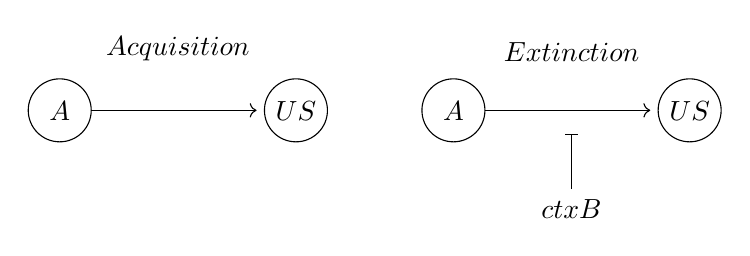
\begin{tikzpicture}
 	%A stage 2
 	\draw(7,2) circle(0.4);
 	\coordinate [label=$A$] (A) at (7, 1.75);
 	\draw[->](7.4,2) -- (9.5,2);
 	\draw(10,2) circle(0.4);
 	\draw[-|](8.5,1) -- (8.5,1.7);
 	\coordinate [label=$ctxB$] (B) at (8.5,0.5);
 	%A stage 1
 	\draw(2,2) circle(0.4);
 	\coordinate [label=$A$] (A) at (2, 1.75);
 	\draw[->](2.4,2) -- (4.5,2);
 	\draw(5,2) circle(0.4);
 	\coordinate [label=$US$] (X1) at (5, 1.75);
 	\coordinate [label=$Acquisition$] (S1) at (3.5,2.5);
 	\coordinate [label=$US$] (X1) at (10, 1.75);
 	\coordinate [label=$Extinction$] (S1) at (8.5,2.5);
 	\end{tikzpicture} } \\
 &
 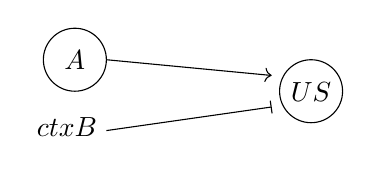
\begin{tikzpicture}
 %A stage 2
 \draw(7,2.4) circle(0.4);
 \coordinate [label=$A$] (A) at (7, 2.15);
 \coordinate [label=$US$] (X1) at (10, 1.75);
 \draw[->](7.4,2.4) -- (9.5,2.2);
 \coordinate [label=$ctxB$] (B) at (6.9,1.3);
 \draw[-|](7.4,1.5) -- (9.5,1.8);
 \draw(10,2) circle(0.4);
 \end{tikzpicture} \\
 \hline
 \end{tabular}
 \captionof{figure}{Illustration of first order and second order associative structures formed during acquisition and extinction (ctxB=context B). The \rwm model suggests first order associations are formed during extinction (bottom-right) whereas an occasion setting model suggests second order associations are formed (top-right). See introductory text starting on pages \pageref{lab:extstr}-\pageref{lab:extstr1} for further details.}
 \label{fig:extinctionStructures}
 \end{table}
 
 \begin{figure}[h]
  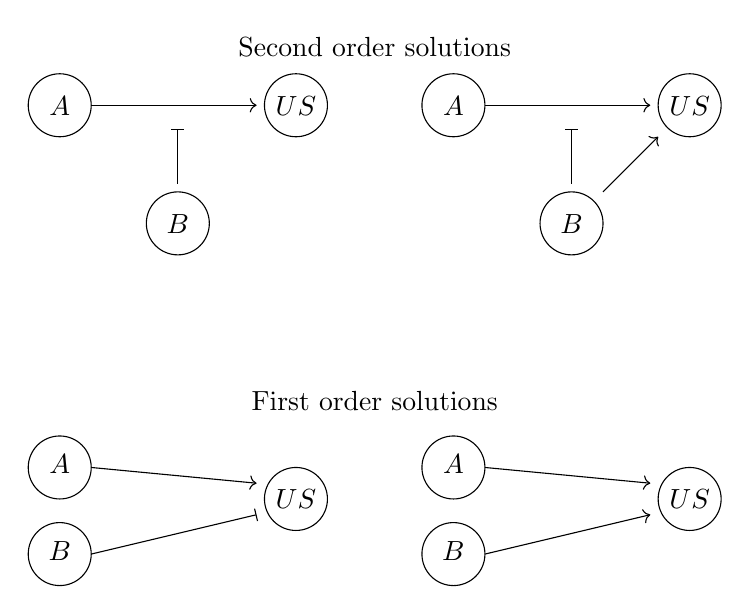
\begin{tikzpicture}
 %LHS top
    \draw(2,7) circle(0.4);
    \coordinate [label=$A$] (A) at (2, 6.75);
    \draw[->](2.4,7) -- (4.5,7);
    \draw(5,7) circle(0.4);
    \coordinate [label=$US$] (US) at (5, 6.75);
    \draw[-|](3.5,6) -- (3.5,6.7);
    \coordinate [label=$B$] (B) at (3.5,5.25);
    \draw(3.5,5.5) circle(0.4);
    \coordinate [label=Second order solutions] (S1) at (6,7.5);
 %LHS bottom
    \coordinate [label=First order solutions] (S1) at (6,3);
       \draw(2,2.4) circle(0.4);
       \coordinate [label=$A$] (A) at (2, 2.2);
       \coordinate [label=$US$] (US) at (5, 1.75);
       \draw[->](2.4,2.4) -- (4.5,2.2);
       \coordinate [label=$B$] (B) at (2,1.1);
       \draw(2,1.3) circle(0.4);
       \draw[-|](2.4,1.3) -- (4.5,1.8);
       \draw(5,2) circle(0.4);
       
 %RHS top
    \draw(7,7) circle(0.4);
    \coordinate [label=$A$] (A) at (7, 6.75);
    \draw[->](7.4,7) -- (9.5,7);
    \draw(10,7) circle(0.4);
    \coordinate [label=$US$] (US) at (10, 6.75);
    \draw[-|](8.5,6) -- (8.5,6.7);
    \coordinate [label=$B$] (B) at (8.5,5.25);
    \draw[->](8.9,5.9) -- (9.6,6.6);
    \draw(8.5,5.5) circle(0.4);
 %RHS bottom
       \draw(7,2.4) circle(0.4);
       \coordinate [label=$A$] (A) at (7, 2.2);
       \coordinate [label=$US$] (US) at (10, 1.75);
       \draw[->](7.4,2.4) -- (9.5,2.2);
       \coordinate [label=$B$] (B) at (7,1.1);
       \draw(7,1.3) circle(0.4);
       \draw[->](7.4,1.3) -- (9.5,1.8);
       \draw(10,2) circle(0.4);
    
  \end{tikzpicture}
  \caption{Status of first and second-order associative structures following training in a feature negative discrimination (left-hand side) and after reinforcement of the feature, B+ trials (right-hand side). See introductory text starting on page \pageref{lab:extstr1} for further details} \label{fig:reversalStructures}
  \end{figure}
  
\clearpage
\begin{figure}[ht]
	\begin{center}
		\begin{subfigure}[b]{0.45\textwidth}
\begin{knitrout}
\definecolor{shadecolor}{rgb}{0.969, 0.969, 0.969}\color{fgcolor}
\includegraphics[width=\maxwidth]{figure/TRACEAoE1-1} 

\end{knitrout}
			\caption{Experiment 1: Cue A} \label{fig:AtraceE1}
		\end{subfigure}
		\begin{subfigure}[b]{0.45\textwidth}
\begin{knitrout}
\definecolor{shadecolor}{rgb}{0.969, 0.969, 0.969}\color{fgcolor}
\includegraphics[width=\maxwidth]{figure/TRACEGoE1-1} 

\end{knitrout}
			\caption{Cue G} \label{fig:GtraceE1}
		\end{subfigure} \\
		\begin{subfigure}[b]{0.45\textwidth}
\begin{knitrout}
\definecolor{shadecolor}{rgb}{0.969, 0.969, 0.969}\color{fgcolor}
\includegraphics[width=\maxwidth]{figure/TRACEAoE2-1} 

\end{knitrout}
			\caption{Experiment 2: Cue A} \label{fig:AtraceE2}
		\end{subfigure}
		\begin{subfigure}[b]{0.45\textwidth}
\begin{knitrout}
\definecolor{shadecolor}{rgb}{0.969, 0.969, 0.969}\color{fgcolor}
\includegraphics[width=\maxwidth]{figure/TRACEGoE2-1} 

\end{knitrout}
			\caption{Cue G} \label{fig:GtraceE2}
		\end{subfigure} \\
\caption{Experiments 1 and 2 x-responses to cues A and G during acquisition, extinction, summation, and recovery test phases. Means $\pm$ 1 standard error.}
	\label{fig:aqexrt}
	\end{center}
\end{figure}

\clearpage
\begin{figure}[ht]
\begin{center}
\begin{subfigure}[b]{0.45\textwidth}
\begin{knitrout}
\definecolor{shadecolor}{rgb}{0.969, 0.969, 0.969}\color{fgcolor}
\includegraphics[width=\maxwidth]{figure/FNE1-1} 

\end{knitrout}
\caption{Experiment 1: training} \label{fig:FNE1}
\end{subfigure}
\begin{subfigure}[b]{0.45\textwidth}
\begin{knitrout}
\definecolor{shadecolor}{rgb}{0.969, 0.969, 0.969}\color{fgcolor}
\includegraphics[width=\maxwidth]{figure/FNRE1-1} 

\end{knitrout}
\caption{reversal} \label{fig:FNRE1}
\end{subfigure} \\
\begin{subfigure}[b]{0.45\textwidth}
\begin{knitrout}
\definecolor{shadecolor}{rgb}{0.969, 0.969, 0.969}\color{fgcolor}
\includegraphics[width=\maxwidth]{figure/FNE2-1} 

\end{knitrout}
\caption{Experiment 2: training} \label{fig:FNE2}
\end{subfigure}
\begin{subfigure}[b]{0.45\textwidth}
\begin{knitrout}
\definecolor{shadecolor}{rgb}{0.969, 0.969, 0.969}\color{fgcolor}
\includegraphics[width=\maxwidth]{figure/FNRE2-1} 

\end{knitrout}
\caption{reversal} \label{fig:FNRE2}
\end{subfigure} \\
\caption{Experiments 1 and 2 outcome-likelihood ratings during feature negative training and feature reversal phases. Means $\pm$ 1 standard error.}
\label{fig:fnfnr}
\end{center}
\end{figure}

\clearpage
\begin{figure}[ht]
\begin{center}
\begin{subfigure}[b]{0.45\textwidth}
\begin{knitrout}
\definecolor{shadecolor}{rgb}{0.969, 0.969, 0.969}\color{fgcolor}
\includegraphics[width=\maxwidth]{figure/FNTE1-1} 

\end{knitrout}
\caption{Experiment 1} \label{fig:FNTE1}
\end{subfigure}
\begin{subfigure}[b]{0.45\textwidth}
\begin{knitrout}
\definecolor{shadecolor}{rgb}{0.969, 0.969, 0.969}\color{fgcolor}
\includegraphics[width=\maxwidth]{figure/FNTE2-1} 

\end{knitrout}
\caption{Experiment 2} \label{fig:FNTE2}
\end{subfigure} \\
\caption{Experiments 1 and 2 test for survival of feature negative discrimination following feature reversal. Means $\pm$ 1 standard error.}
\label{fig:fnt}
\end{center}
\end{figure}

\clearpage
\begin{figure}[ht]
\begin{center}
\begin{subfigure}[b]{0.45\textwidth}
\begin{knitrout}
\definecolor{shadecolor}{rgb}{0.969, 0.969, 0.969}\color{fgcolor}
\includegraphics[width=\maxwidth]{figure/InTestE1-1} 

\end{knitrout}
\caption{Experiment 1} \label{fig:INTE1}
\end{subfigure}
\begin{subfigure}[b]{0.45\textwidth}
\begin{knitrout}
\definecolor{shadecolor}{rgb}{0.969, 0.969, 0.969}\color{fgcolor}
\includegraphics[width=\maxwidth]{figure/InTestE2-1} 

\end{knitrout}
\caption{Experiment 2} \label{fig:INTE2}
\end{subfigure} \\
\begin{subfigure}[b]{0.9\textwidth}
\begin{knitrout}
\definecolor{shadecolor}{rgb}{0.969, 0.969, 0.969}\color{fgcolor}
\includegraphics[width=\maxwidth]{figure/InTestsAll-1} 

\end{knitrout}
\caption{Combined Experiments 1 and 2} \label{fig:INTALL}
\end{subfigure} \\
\caption{Top. Experiments 1 and 2 responses to AB compound in feature negative survival test for participants classified as non-inhibitors and inhibitors. Bottom. Data combined over Experiments 1 and 2. Means $\pm$ 1 standard error.}
\label{fig:inht}
\end{center}
\end{figure}

\clearpage
\def\ms{15mm}
\def\plw{20mm}
\def\plh{20mm}
\begin{table}[t]
\begin{tabular}{lc}
\hline
\multirow{13}{*}{
	\begin{tikzpicture}[baseline=(current bounding box.north),
	ocircle/.style={circle,draw,minimum size=\ms},
	odcircle/.style={circle,draw,minimum size=\ms,double, double distance=2pt},
	shcircle/.style={circle,draw,minimum size=\ms,fill=black!20},
	orect/.style={rectangle,draw,minimum size=\ms},
	shrect/.style={rectangle,draw,minimum size=\ms,fill=black!20},
	plate/.style={rectangle, draw, rounded corners=3mm,minimum width=\plw, minimum height=\plh}]
	\node(p1) at (0,0) [plate,label=below:NoInh data]{};
	\node (xi) at (0,0) [shcircle] {\Large{$x_i$}};
	\node(p2) at (3,0) [plate,label=below:Inh data]{};
	\node (yj) at (3,0) [shcircle] {\Large{$y_j$}};
	\node (mu) at (-0.5,3)[ocircle]{\Large{$\mu$}}; 
	\node (sig) at (3.5,3)[ocircle]{\Large{$\sigma$}}; 
	\node (delta) at (1.5,4)[ocircle]{\Large{$\delta$}}; 
	\node (sigMu) at (-0.5,5.5)[odcircle]{\Large{$\sigma_\mu$}};
	\node (sigDelta) at (1.5,7)[odcircle]{\Large{$\sigma_\delta$}}; 
	\draw[-{>[scale=2.5,
		length=2,
		width=3]}](mu)--(xi);
	\draw[-{>[scale=2.5,
		length=2,
		width=3]}](mu)--(yj);
	\draw[-{>[scale=2.5,
		length=2,
		width=3]}](sig)--(xi);
	\draw[-{>[scale=2.5,
		length=2,
		width=3]}](sig)--(yj);
	\draw[-{>[scale=2.5,
		length=2,
		width=3]}](delta)--(yj);
	\draw[-{>[scale=2.5,
		length=2,
		width=3]}](sigMu)--(mu);
	\draw[-{>[scale=2.5,
		length=2,
		width=3]}](sigDelta)--(delta);
	\end{tikzpicture}} & \\   &  \\ & \\
& $\sigma_\delta \leftarrow 100 \times \sqrt{2} \times \sigma_{xy}$ \\
& $\sigma_\mu \leftarrow 100 \times \sigma_{xy}$ \\
& $\delta \sim$ Gaussian(0, $\sfrac{1}{\sigma_\delta^2}$)\\
& $\mu \sim$ Gaussian($\mu_{x}$,$\sfrac{1}{\sigma_\mu^2}$) \\
& $\sigma \sim$ Uniform($\sigma_{xy} \times \sfrac{1}{100}$, $\sigma_{xy} \times 100$) \\
& $x_i \sim$ Gaussian($\mu$, $\sfrac{1}{\sigma^2}$) \\
& $y_j \sim$ Gaussian($\mu+\delta$, $\sfrac{1}{\sigma^2}$) \\
& \\   & \\  & \\   & \\  
\hline \vspace{2pt}
\end{tabular}
\captionof{figure}{Graphical model for Analysis 1. $\sigma_{xy}$ is pooled standard deviation of observed data from both groups, $\mu_{x}$ is the mean of the data from the non-inhibitors group. The parameterisation of Gaussian distributions in JAGS is in terms of mean and precision where precision is $\sfrac{1}{\sigma^2}$}.
\label{tab:gm1}
\end{table}

\clearpage
\begin{figure}[ht]
\begin{center}
\begin{knitrout}
\definecolor{shadecolor}{rgb}{0.969, 0.969, 0.969}\color{fgcolor}
\includegraphics[width=\maxwidth]{figure/pltB2-1} 

\end{knitrout}
\caption{Jittered raw data and posterior distributions for the ratings given by the non-inhibitors and inhibitors in the AB compound test. The region of practical equivalence and the 95\% Bayesian credible interval are given around the means of the distributions for the non-inhibitors and the inhibitors, respectively.} 
\label{fig:posteriors}
\end{center}
\end{figure}


\begin{table}[t]
\begin{tabular}{lc}
\hline
\multirow{13}{*}{
	\begin{tikzpicture}[baseline=(current bounding box.north),
	ocircle/.style={circle,draw,minimum size=\ms},
	odcircle/.style={circle,draw,minimum size=\ms,double, double distance=2pt},
	shcircle/.style={circle,draw,minimum size=\ms,fill=black!20},
	orect/.style={rectangle,draw,minimum size=\ms},
	shrect/.style={rectangle,draw,minimum size=\ms,fill=black!20},
	plate/.style={rectangle, draw, rounded corners=3mm,minimum width=\plw, minimum height=\plh}]
	\node(p1) at (0,0) [plate,label=below:NoInh data]{};
	\node (xi) at (0,0) [shcircle] {\Large{$x_i$}};
	\node(p2) at (3,0) [plate,label=below:Inh data]{};
	\node (yj) at (3,0) [shcircle] {\Large{$y_j$}};
	\node (mu) at (-0.5,3)[ocircle]{\Large{$\mu$}}; 
	\node (sigma) at (3.5,3)[ocircle]{\Large{$\sigma$}}; 
	\node (alpha) at (1.5,4)[odcircle]{\Large{$\alpha$}}; 
	\node (delta) at (1.5,7)[ocircle]{\Large{$\delta$}}; 
	\draw[-{>[scale=2.5,
		length=2,
		width=3]}](mu)--(xi);
	\draw[-{>[scale=2.5,
		length=2,
		width=3]}](mu)--(yj);
	\draw[-{>[scale=2.5,
		length=2,
		width=3]}](sigma)--(xi);
	\draw[-{>[scale=2.5,
		length=2,
		width=3]}](sigma)--(yj);
	\draw[-{>[scale=2.5,
		length=2,
		width=3]}](alpha)--(yj);
	\draw[-{>[scale=2.5,
		length=2,
		width=3]}](sigma)--(alpha);
	\draw[-{>[scale=2.5,
		length=2,
		width=3]}](delta)--(alpha);
	\end{tikzpicture}} & \\   &  \\ & \\
& $\delta \sim$ Cauchy(0,1) \\
& $\mu \sim$ Cauchy(0,1) \\
& $\alpha \leftarrow \delta \sigma$ \\
& $\sigma \sim$ Cauchy(0,1)$[0,\infty]$ \\
& $x_i \sim$ Gaussian($\mu$, $\sfrac{1}{\sigma^2}$) \\
& $y_j \sim$ Gaussian($\mu+\alpha$, $\sfrac{1}{\sigma^2}$) \\
& \\   & \\  & \\   & \\  
\hline \vspace{2pt}
\end{tabular}
\captionof{figure}{Graphical model for Analysis 2. The parameterisation of Gaussian distributions in JAGS is in terms of mean and precision where precision is $\sfrac{1}{\sigma^2}$}
\label{tab:gm2}
\end{table}

\clearpage
\begin{figure}[ht]
\begin{center}
\begin{knitrout}
\definecolor{shadecolor}{rgb}{0.969, 0.969, 0.969}\color{fgcolor}
\includegraphics[width=\maxwidth]{figure/pltB1-1} 

\end{knitrout}
\caption{Prior and posterior distributions for the effect size ($\delta$) on the difference between the group means for non-inhibitors and inhibitors in the AB compound test. The relative values of the distributions is given at $\delta =0$ and the 95\% Bayesian credible interval is given around the mean of the posterior distribution.} 
\label{fig:effectsizes}
\end{center}
\end{figure}

\end{document}
